\documentclass[border=2pt]{standalone}
\usepackage{times,tikz}
\usetikzlibrary{arrows.meta,positioning,fit}
\begin{document}
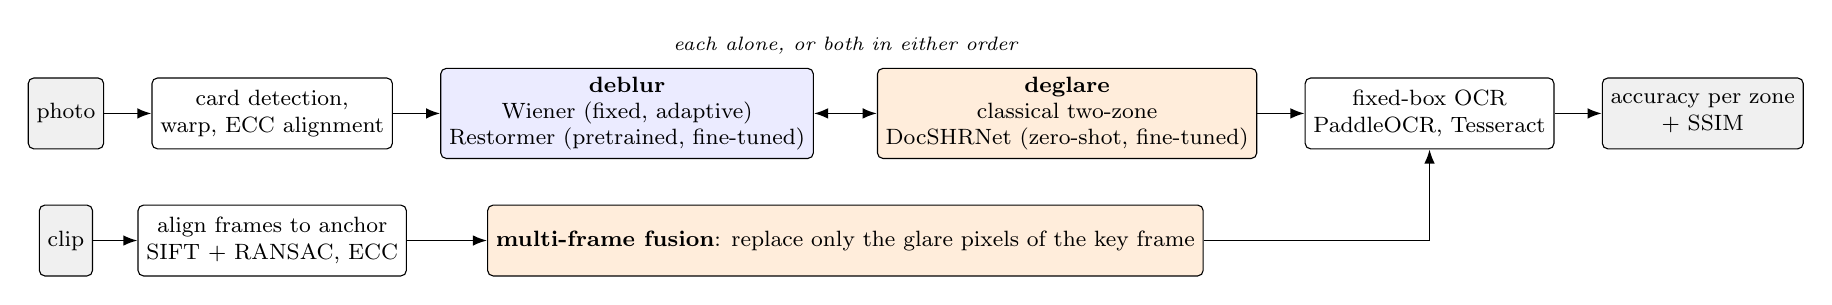
\begin{tikzpicture}[font=\footnotesize, node distance=5mm and 6mm,
  box/.style={draw,rounded corners=2pt,align=center,minimum height=9mm,inner sep=3pt,fill=white},
  data/.style={box,fill=black!6}, blur/.style={box,fill=blue!8}, glare/.style={box,fill=orange!14},
  arr/.style={-{Latex[length=1.8mm]},semithick}]
% single photo
\node[data] (in) {photo};
\node[box,right=of in] (rect) {card detection,\\warp, ECC alignment};
\node[blur,right=of rect] (blur) {\textbf{deblur}\\Wiener (fixed, adaptive)\\Restormer (pretrained, fine-tuned)};
\node[glare,right=8mm of blur] (glare) {\textbf{deglare}\\classical two-zone\\DocSHRNet (zero-shot, fine-tuned)};
\node[box,right=of glare] (ocr) {fixed-box OCR\\PaddleOCR, Tesseract};
\node[data,right=of ocr] (ev) {accuracy per zone\\+ SSIM};
\draw[arr] (in)--(rect); \draw[arr] (rect)--(blur); \draw[arr] (glare)--(ocr); \draw[arr] (ocr)--(ev);
\draw[{Latex[length=1.8mm]}-{Latex[length=1.8mm]},semithick] (blur)--(glare);
\node[above=0.5mm of blur.north east,xshift=4mm,font=\scriptsize\itshape] {each alone, or both in either order};
% clip
\node[data,below=7mm of in] (clip) {clip};
\node[box] (al) at (clip -| rect) {align frames to anchor\\SIFT + RANSAC, ECC};
\path (blur) -- (glare) coordinate[midway] (mid);
\node[glare] (fuse) at (al -| mid) {\textbf{multi-frame fusion}: replace only the glare pixels of the key frame};
\draw[arr] (clip)--(al); \draw[arr] (al)--(fuse); \draw[arr] (fuse.east) -| (ocr.south);
\end{tikzpicture}
\end{document}
